\documentclass{beamer}
\usepackage{amsmath}
\usepackage{latexsym}
\usepackage{graphicx}
\usepackage{sidecap}
\usepackage{stmaryrd}
\usepackage{pdfpages}
\usepackage{wrapfig}

\mode<presentation> {
\usetheme{Dresden}
\usecolortheme{lily}
\setbeamertemplate{navigation symbols}{} 
}

\usepackage{graphicx} 
\usepackage{booktabs} 

%----------------------------------------------------------------------------------------
%	TITLE PAGE
%----------------------------------------------------------------------------------------

\title[Quotient Containers in Homotopy Type Theory]{Quotient Containers in Homotopy Type Theory} % The short title appears at the bottom of every slide, the full title is only on the title page

\author{\textbf{Jonathan Sherry}} % Your name
\institute[University of Nottingham] % Your institution as it will appear on the bottom of every slide, may be shorthand to save space
{
\small{Supervisor: Thorsten Altenkirch}\\
University of Nottingham  % Your institution for the title page
}
\date{27\textsuperscript{th} November  2013 } % Date, can be changed to a custom date

\begin{document}

\begin{frame}
\titlepage
\end{frame}


%----------------------------------------------------------------------------------------
%	PRESENTATION SLIDES
%----------------------------------------------------------------------------------------

\begin{frame}
\frametitle{Homotopy Type Theory}
\begin{columns}[c]

\column{.5\textwidth}
\begin{itemize}
\item \scriptsize{Developed by \textit{Univalent Foundations Program} at the Institute of Advanced Study, Princeton (Steve Awodey, Thierry Coquand and Vladimir Voevodsky et al.)}
\item \scriptsize{Gives homotopical meaning to ideas in Martin-L\"of Type Theory}
\end{itemize}

\column{.4\textwidth}
\begin{flushleft}

\includegraphics[scale=0.23]{1.png}
\end{flushleft}


\end{columns}

\end{frame}

%-----------------------------------------------------

\begin{frame}
\frametitle{Key Ideas in HoTT}
\begin{columns}[c]

\column{.5\textwidth}
\begin{itemize}
\item Terms of a type are points in a space
\item A function $ f : A \to B $ is a continuous mapping from space $ A $ to space $ B $
\item If $a = b$ for $a,b : A$ then a path $ p : a \leadsto b $ exists between a and b in A
\item Two functions $ f,g : A \to B $ can be identified if they are homotopic (i.e. one can be continuously deformed onto another)
\end{itemize}

\column{.5\textwidth}
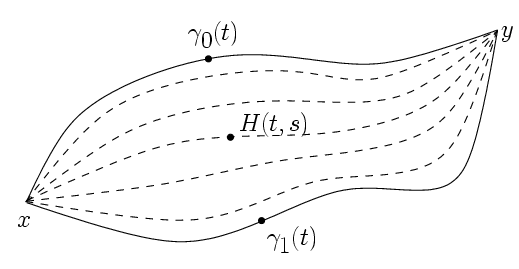
\includegraphics[scale=0.3]{./2.png}\\
\small{\textit{Homotopy between two curves: the curves $\gamma_0$ and $ \gamma_1$ are homotopic by the homotopy $H$}}


\end{columns}
\end{frame}

%-----------------------------------------------------

\begin{frame}
\frametitle{HoTT vs MLTT}

\begin{itemize}
\item Different notion of equality in homotopy type theory
\item Allows representation of multisets (bags)
\item Cannot be represented in conventional type theory 
\end{itemize}
\end{frame}



%------------------------------------------------

\begin{frame}
\frametitle{Containers}
\begin{itemize}
\item Type theoretic abstraction for collection types (lists, queues, trees etc)
\item Allows these types to be represented in  a uniform manner
\item Unary container is defined as a pair $ (S \rhd P)$ such that $ S : Set $ and $ P : S \to Set $
\item Elements of the set S are \textit{shapes} of the container
\item Elements of $P(s)$ are the \textit{positions} of s for $ s : S $
\item Can be evaluated as an endofunctor
\end{itemize}
\end{frame}

%------------------------------------------------

\begin{frame}[fragile]
\frametitle{List Container}
List Definition:
\begin{verbatim}
     data List (A : Set) : Set where
          Nil : List A
          Cons : A -> List A -> List A
\end{verbatim}
would have the form $ (S \rhd P)$ such that $ S = \mathbb{N} $ and $ P = Fin $
\end{frame}

%------------------------------------------------

\begin{frame}
\frametitle{Category of Containers}

Container endofunctor:\\
\begin{center}
$\llbracket S \rhd P\rrbracket \in Set \to Set$\\
$ \llbracket S \rhd P\rrbracket X = \Sigma s \in S. P s \to X $\\
\end{center}
\smallskip
Given containers $ (S \rhd P)$ and $ (T \rhd Q)$, morphism $ f \rhd r $ is given by:\\
\medskip
\begin{center}
$f \in S \to T$\\
$r \in \Pi _{s \in S} Q(f s) \to P s $\\
\end{center}
Gives rise to natural transformations.


\end{frame}

%------------------------------------------------

\begin{frame}
\frametitle{Aims and Objectives}
\begin{enumerate}
\item To research and understand Homotopy Type Theory
\item To research and understand Quotient Containers and their applications
\item To formalise the notion of Quotient Containers within the context of Homotopy Type Theory
\item To potentially explore applications of Quotient Containers within the context of Homotopy Type Theory
\item To potentially explore interesting or novel theorems surrounding Quotient Containers in Homotopy Type Theory
\end{enumerate}
\end{frame}

%------------------------------------------------

\begin{frame}
\frametitle{Project Plan}
\fontsize{7.5pt}{7.2}\selectfont
\begin{center}
\begin{tabular}{l l}

 \textbf{25 October - 20 November 2013} & Ongoing research into HoTT and Quotient Containers \\
 \textbf{25 October - 20 November 2013} & Ongoing learning of Agda \\
 \textbf{20 November - 26 November 2013} & Preparation for presentation \\
 \textit{\textbf{27 November 2013}} & Presentation of progress \\
 \textbf{28 November - 31 January 2014} & Continued relevant and more focussed research  \\
 \textbf{01 February - 24 February 2014} & Writing of dissertation outline and sample chapter \\

 \textbf{25 February - 27 February 2014} & Proof read/copy edit/typeset sample chapter \\
 \textit{\textbf{28 February 2014}} & Submission of dissertation outline and sample chapter \\
 \textbf{31 March 2014} & Complete first draft of dissertation \\
 \textbf{01 April - 31 April 2014} & Redraft and rewrite dissertation \\
 \textbf{31 April 2014} & \underline{Complete dissertation} \\
 \textbf{01 May - 11 May 2014} & Final checks and typesetting of dissertation \\
 \textbf{01 May - 13 May 2014} & Preparation for demonstration of project \\
 \textit{\textbf{12 May 2014}} & Submission of complete dissertation \\
 \textit{\textbf{14 May 2014}} & Demonstration of project \\

\end{tabular}
\end{center}
\end{frame}

%------------------------------------------------

\begin{frame}
\frametitle{Progress}
\begin{block}{Research}
\begin{itemize}
\item Homotopy Type Theory
\begin{itemize}
\item HoTT Book
\item http://homotopytypetheory.org
\end{itemize}
\item Containers
\begin{itemize}
\item Hakon Robbestad Gylterud - Symmetric Containers
\item Abbott, Altenkirch, Ghani - Constructing Strictly Positive Types
\item Altenkirch, Levy, Staton - Higher Order Containers
\end{itemize}
\item Agda
\begin{itemize}
\item Agda wiki
\item Francesco Mazzoli - Agda by Example: $\lambda$-calculus
\item Thorsten Altenkirch - Type Theory in Rosario
\end{itemize}
\end{itemize}
\end{block}
\end{frame}

%------------------------------------------------
\begin{frame}
\frametitle{Progress}

\begin{block}{Formalization in Agda}
\begin{itemize}
\item Containers
\item Container morphisms
\item Evaluating containers as functors
\item Container morphisms as natural transformations
\end{itemize}
\end{block}
\end{frame}
%------------------------------------------------

\begin{frame}
\frametitle{Progress}
\begin{block}{Written Dissertation}
\begin{itemize}
\item Abstract
\item Introduction
\item Background Information
\end{itemize}
\end{block}

\end{frame}

\begin{frame}
\begin{center}
Progress can be tracked at:\\
\texttt{https://github.com/jxs1/ids}\\
\bigskip
\Huge{\textit{Questions?}}
\end{center}

\end{frame}

%----------------------------------------------------------------------------------------

\end{document}